\subsection{\emph{ROS 2 Interface}}
\label{subsec:ros2interface}

\emph{ROS 2 interface} merupakan suatu bentuk struktur pesan yang digunakan pada sistem komunikasi yang ada di ROS 2.
\emph{Interface} yang ada di ROS 2 terdiri dari tiga jenis,
  \emph{msg} dengan \emph{file format} \lstinline{.msg} yang digunakan pada \emph{ROS 2 topic},
  \emph{srv} dengan \emph{file format} \lstinline{.srv} yang digunakan pada \emph{ROS 2 service},
  dan \emph{action} dengan \emph{file format} \lstinline{.action} yang digunakan pada \emph{ROS 2 Action}.

\emph{ROS 2 interface} dapat dideskripsikan dalam suatu file yang nantinya akan dikompilasi sesuai dengan format yang dibutuhkan oleh RCL maupun RMW.
Seperti pada potongan kode \ref{lst:msgexample},
  sebuah \emph{file interface} berisi beberapa baris yang menunjukkan tipe data, nama, serta nilai \emph{default} dari setiap \emph{field} yang dimiliki oleh \emph{interface} tersebut.
Sebuah \emph{interface} yang ada di ROS 2 bisa memiliki tipe data yang berasal dari \emph{interface} lain,
  sehingga memungkinkan bentuk \emph{interface} yang lebih kompleks seperti yang digunakan pada \emph{interface} untuk informasi kamera dan data citra.

\lstinputlisting[
  style=code,
  caption={Contoh \emph{file msg} yang mendeskripsikan \emph{interface} untuk \emph{topic}.},
  label={lst:msgexample}
]{kode/msg_example.txt}

Seperti yang dijelaskan pada paragraf sebelumnya,
  \emph{ROS 2 interface} akan dikompilasi menjadi bentuk lain agar bisa digunakan di setiap implementasi yang ada di RCL maupun RMW.
Seperti yang terlihat pada gambar \ref{fig:diagraminterfaceros2},
  sebuah \emph{file} \lstinline{.msg} akan dikompilasi menjadi \emph{file} \lstinline{.idl} yang digunakan oleh implementasi DDS pada RMW,
  serta akan dikompilasi menjadi \emph{struct} dan \emph{class} dari bahasa yang digunakan sebagai implementasi dari \emph{RCL}.
Dengan adanya kompilasi ini,
  isi dari sebuah pesan yang dikirim maupun diterima pada ROS 2 dapat dideskripsikan menggunakan satu format yang nantinya bisa digunakan di semua implementasi RMW maupun RCL.

\begin{sidewaysfigure}
  \centering
  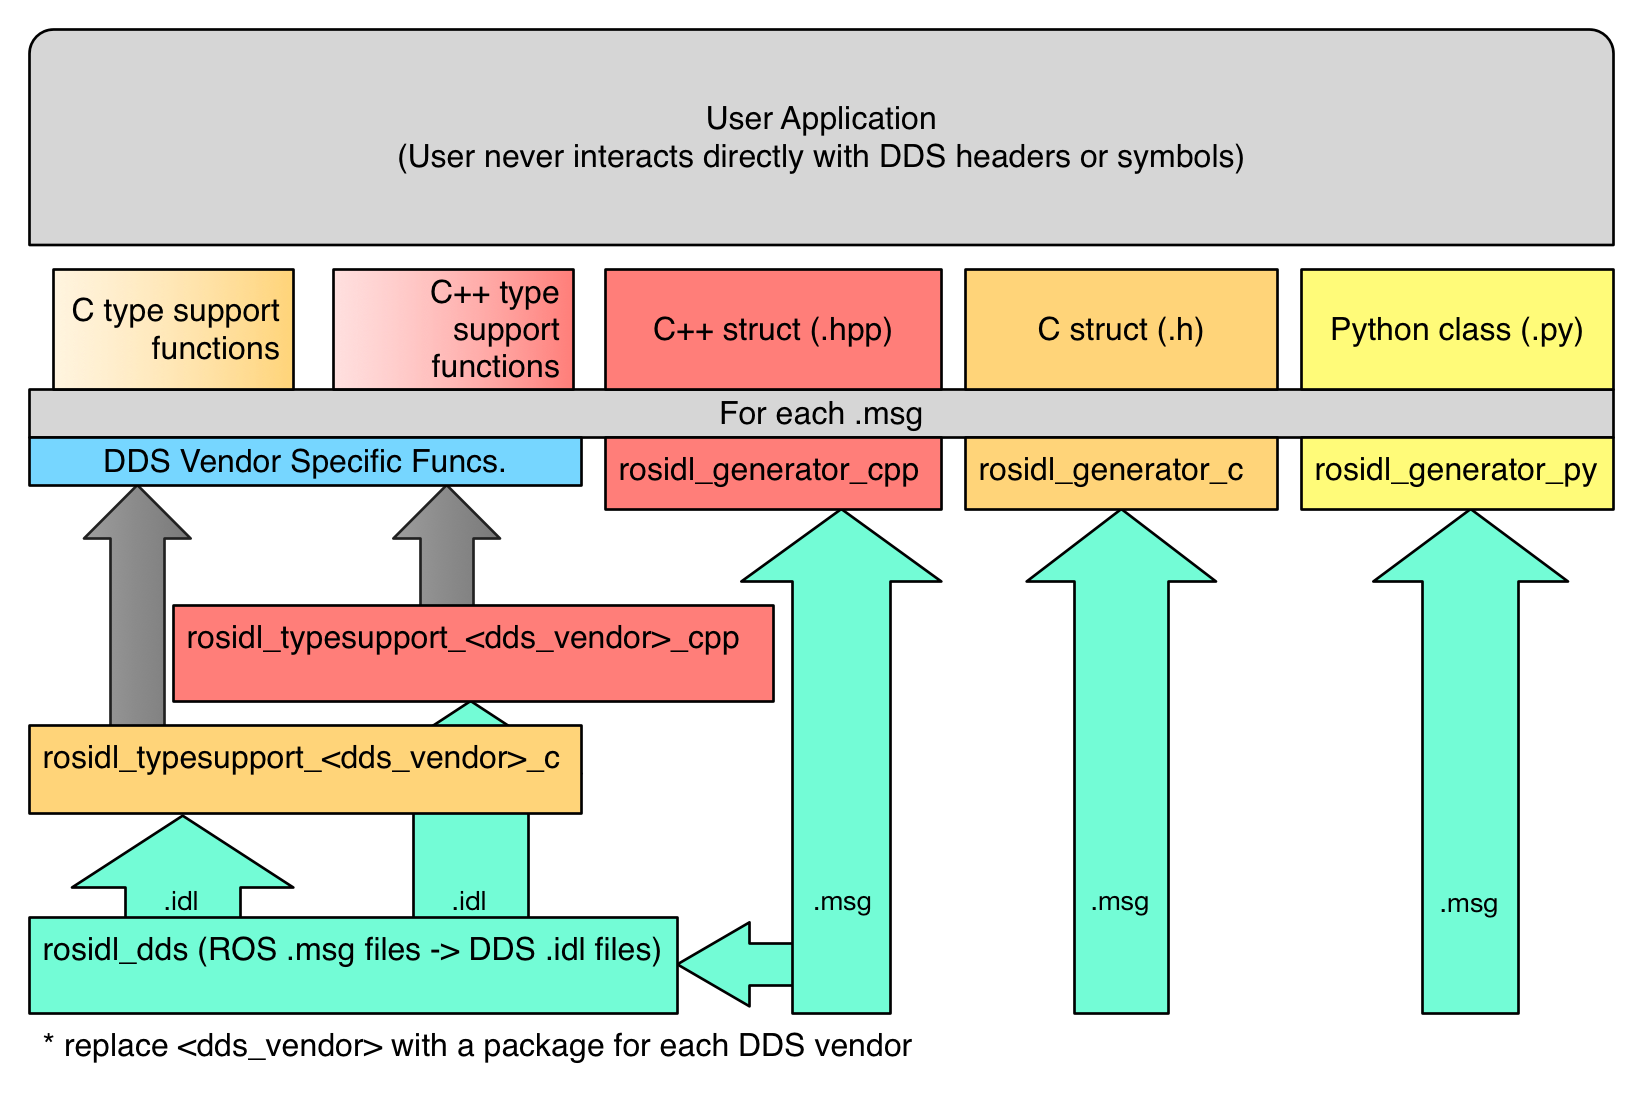
\includegraphics[width=0.8\textwidth,keepaspectratio]{gambar/diagram-interface-ros2.png}
  \caption{Diagram abstraksi interface yang ada pada ROS 2 \citep{url:ros2interfacesconcept}.}
  \label{fig:diagraminterfaceros2}
\end{sidewaysfigure}
